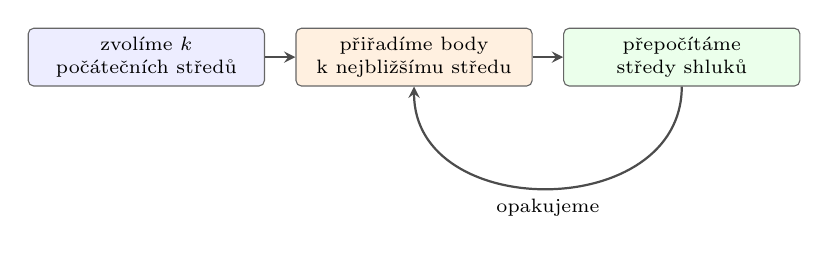
\begin{tikzpicture}[
    >=stealth,
    box/.style={
        draw=black!60,
        rounded corners=2pt,
        minimum width=3.0cm,
        minimum height=0.72cm,
        align=center,
        font=\scriptsize
    },
    arr/.style={->, thick, draw=black!70}
]
    \node[box, fill=blue!7] (start) at (0,0)
        {zvolíme $k$\\počátečních středů};

    \node[box, fill=orange!12] (assign) at (3.4,0)
        {přiřadíme body\\k nejbližšímu středu};

    \node[box, fill=green!8] (update) at (6.8,0)
        {přepočítáme\\středy shluků};

    \draw[arr] (start) -- (assign);
    \draw[arr] (assign) -- (update);
    \draw[arr]
        (update.south)
        to[out=-90,in=-90,looseness=1.3]
        node[below, font=\scriptsize] {opakujeme}
        (assign.south);
\end{tikzpicture}
